
\chapter{Results}

This section summarizes the results and shows rendered images of \lsystems.


\section{Web user interface}

\begin{wrapfigure}{r}{0.4\textwidth}
	
\includegraphics[width=\linewidth]{malsys_cz}
	\caption{\url{http://malsys.cz}}
	\label{fig:malsysQr}
\end{wrapfigure}

The web user interface was deployed and it is accessible at address \url{http://malsys.cz}.
The main function of the web is to process \lsystems.
Detailed instructions can be found in appendix \ref{chap:userDoc}.
Web site includes \lsystem gallery and help.

Any user can register and gain some advantages.
Registered users can save and publish their \lsystems to public gallery and they have longer time limit for processing of \lsystems.

Web page is displayed correctly in the most common web browsers namely Google Chrome, Opera, Firefox, Internet Explorer and Safari.
It is possible to browse it in smart phones or tablets.
\autoref{fig:galleryInDevices} shows print-screens of the first page of the gallery on various operating systems.

If the browser window is wider than 1900 px the layout of the \lsystem process page splits to two columns to allow to see the source code and the result simultaneously.
This feature is done purely in CSS 3.

The web page is supports pinning to the Windows taskbar (\autoref{fig:pinIe}). 

\begin{figure}[h]
	\centering
	\subfloat{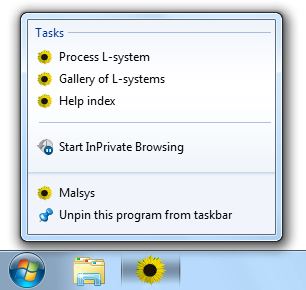
\includegraphics[scale=0.54]{JumpList}} ~
	\subfloat{
\includegraphics[scale=0.7]{PinnedIeHeader}}
	\caption{Jump-list of pinned site and header of opened Internet Explorer 9 using pinned shortcut}
	\label{fig:galleryInDevices}
\end{figure}


\begin{figure}[p]
	\centering
	\subfloat[Windows 7 (Google Chrome)]{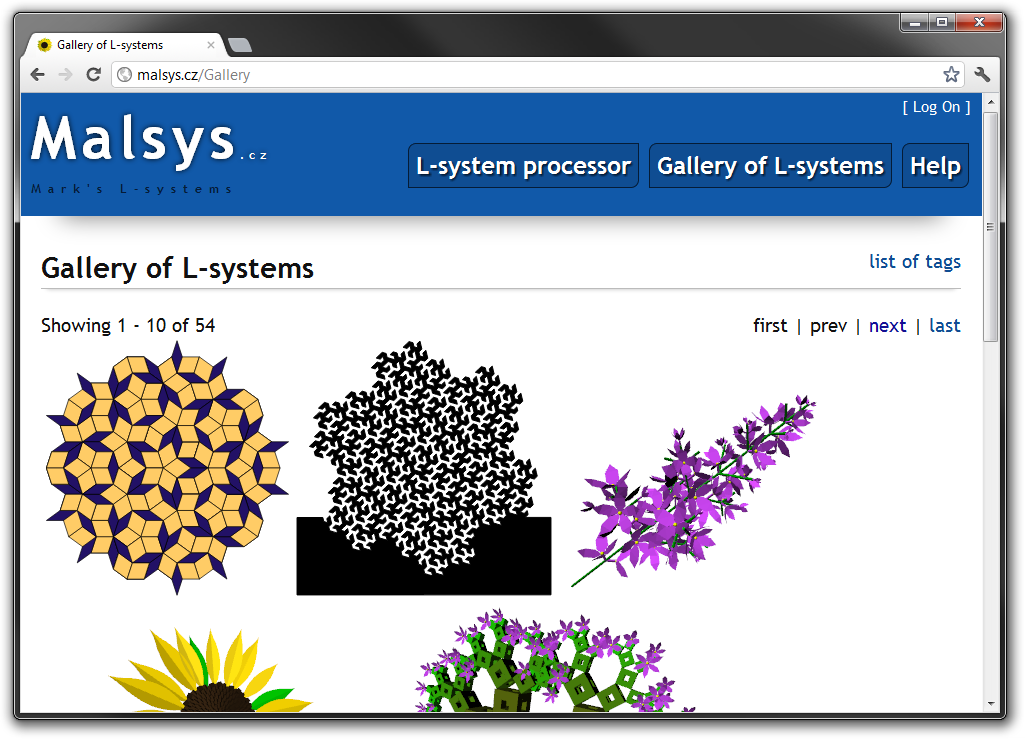
\includegraphics[width=\linewidth]{GalleryInChrome}}
	\\
	\subfloat[Android ICS (default browser)]{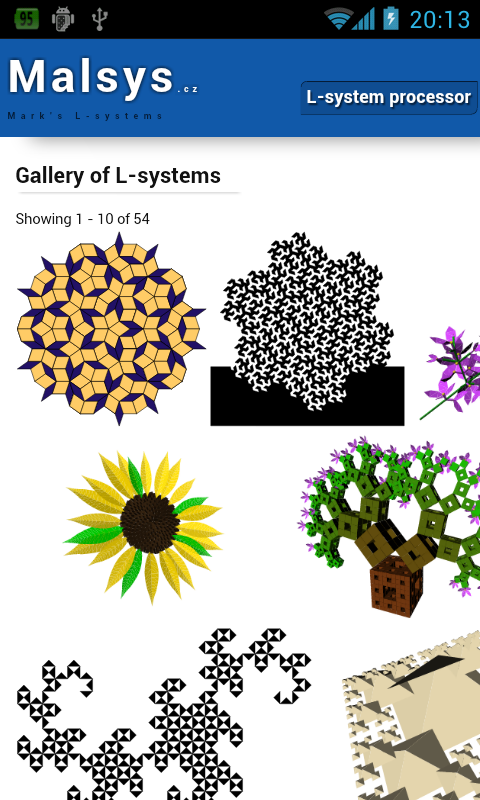
\includegraphics[height=7cm]{GalleryOnAndroid}} ~
	\subfloat[Windows Phone (IE9 mobile)]{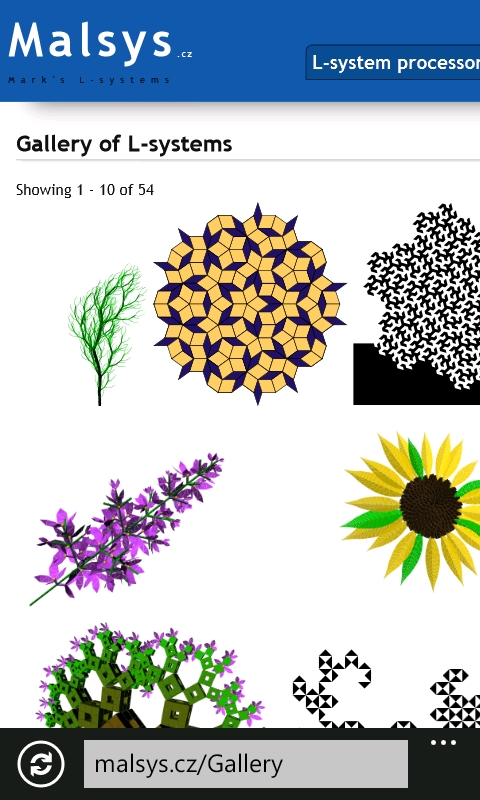
\includegraphics[height=7cm]{GalleryOnWindowsPhone}} ~
	\subfloat[Amazon Kindle 3]{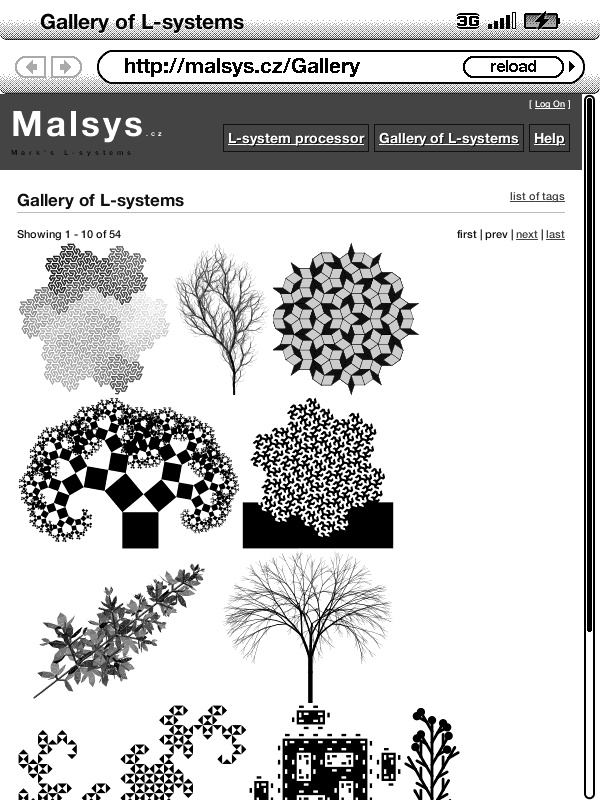
\includegraphics[height=7cm]{GalleryOnKindle}}
	\caption{The first page of the gallery displayed on various operating systems}
	\label{fig:pinIe}
	\nomenclature{IE}{Internet Explorer}
\end{figure}


\subsection{Visitors and traffic}

The web was officially released on 15 April 2012.
Two days later it was posted some notifications on Twitter and Facebook.
This day number of visitors peeked at 142 but most of them just checked the gallery and next day the the messages on social networks were lost.

About week after initial release short newsflash was posted on Czech server \url{http://root.cz} which attracted 255 visitors that day.
But visitors from the root.cz was not just looking in the gallery.
In the contrast with visitors from social networks users from the root.cz started to experiment with \lsystems.
This was probably because of fact that the root.cz is the a site about computer technologies, software and programming and users understood \lsystems better.

At the end of May, one and half months after initial release malsys.cz was seen by over 1000 unique visitors and they browsed over 9000 pages.


\section{Showcase of \lsystems}

The most \lsystems is used in this thesis as figures illustration described themes.
In this section are images of some more \lsystems.

\begin{figure}[h]
	\subfloat{
		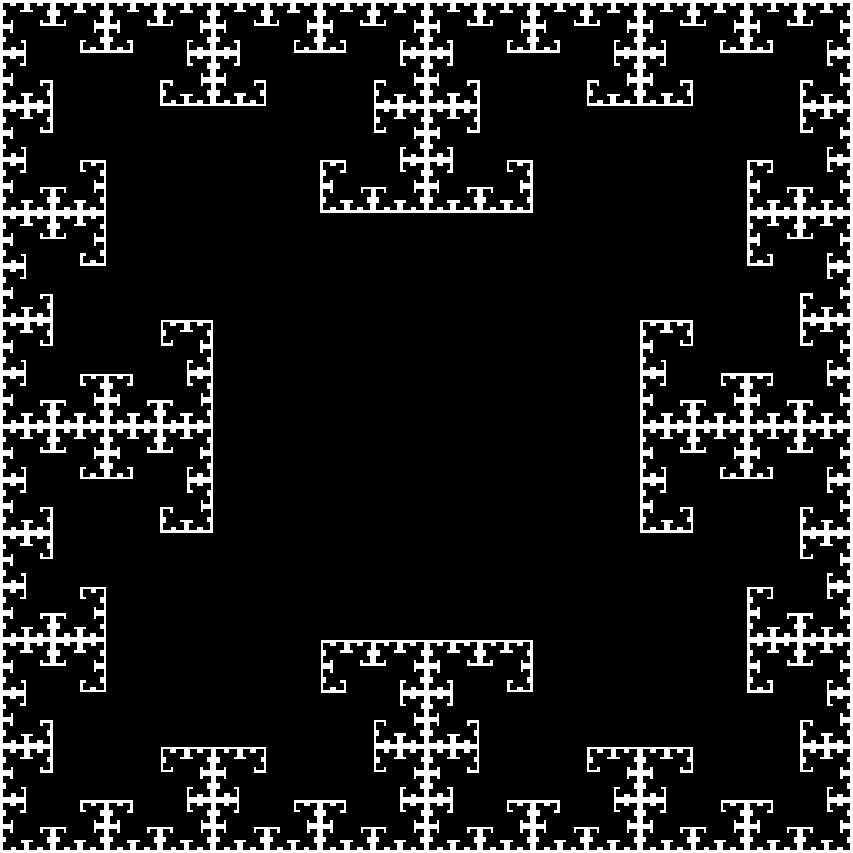
\includegraphics[width=0.49\linewidth]{Tsquare}
		\label{fig:introLilac}
	} \hfill
	\subfloat{
		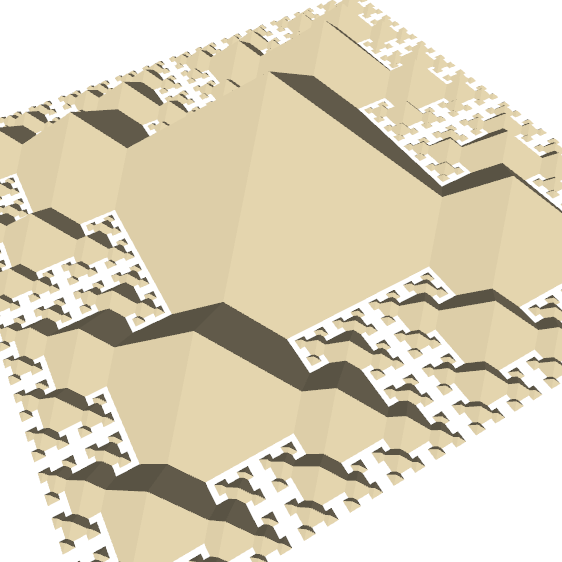
\includegraphics[width=0.49\linewidth]{Tsquare3D}
		\label{fig:introHTree}
	}
	\caption{T-square fractal (left) and its generalization to 3D with pyramids instead of squares (right)}
\end{figure}

\begin{figure}[h]
	\subfloat{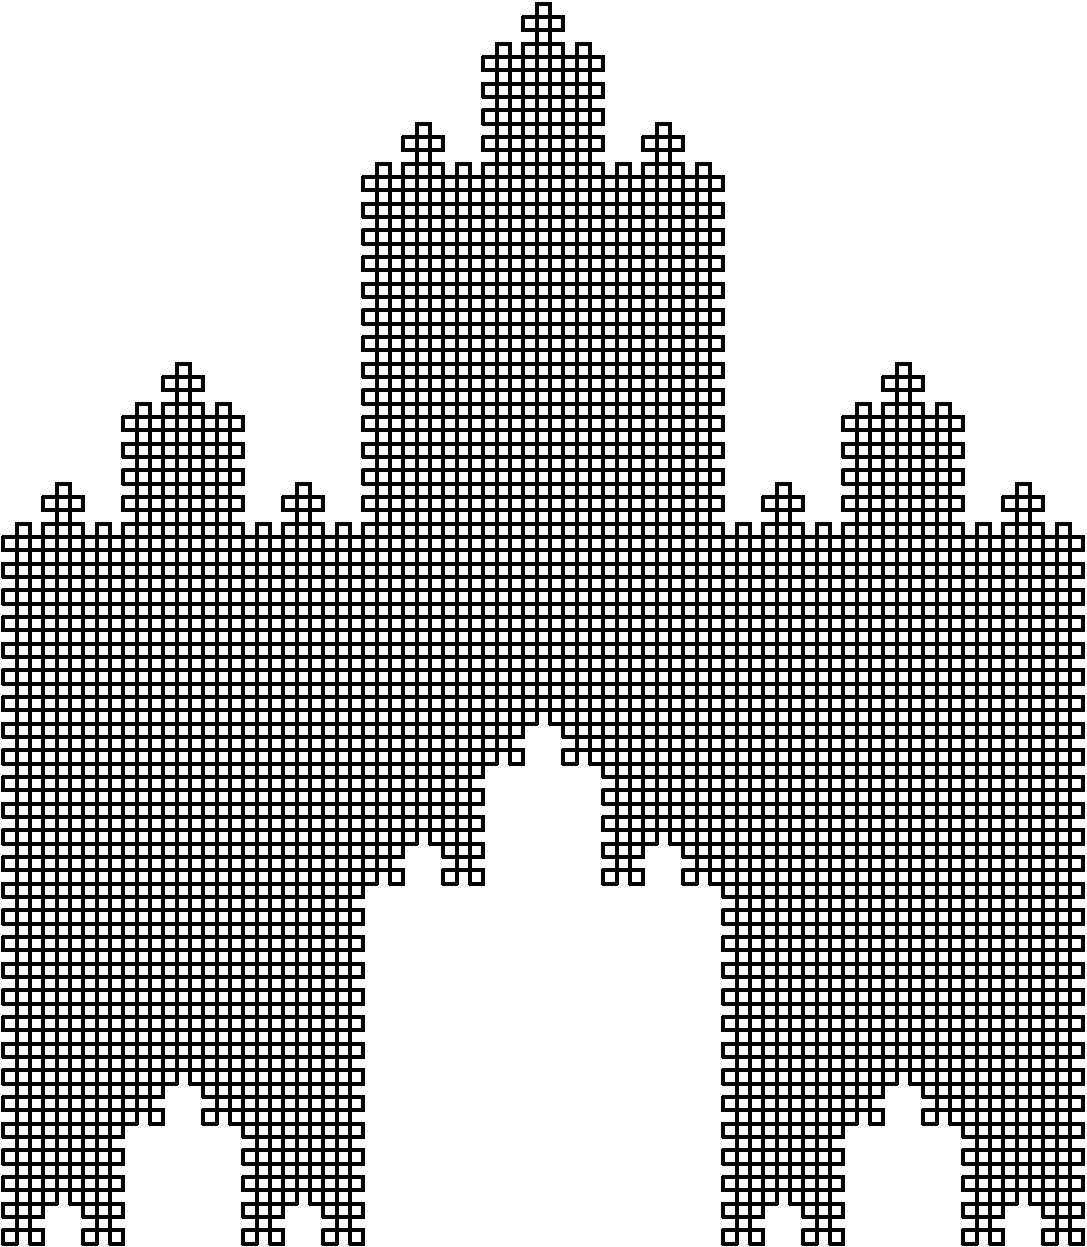
\includegraphics[width=0.49\linewidth]{DekkingsChurch}}
	\hfill
	\subfloat{
\includegraphics[width=0.49\linewidth]{HilbertCurve}}
	\caption{Dekking's chirch (left) and Hilbert curve (right)}
\end{figure}

\begin{figure}[p]
	\centering
	\subfloat{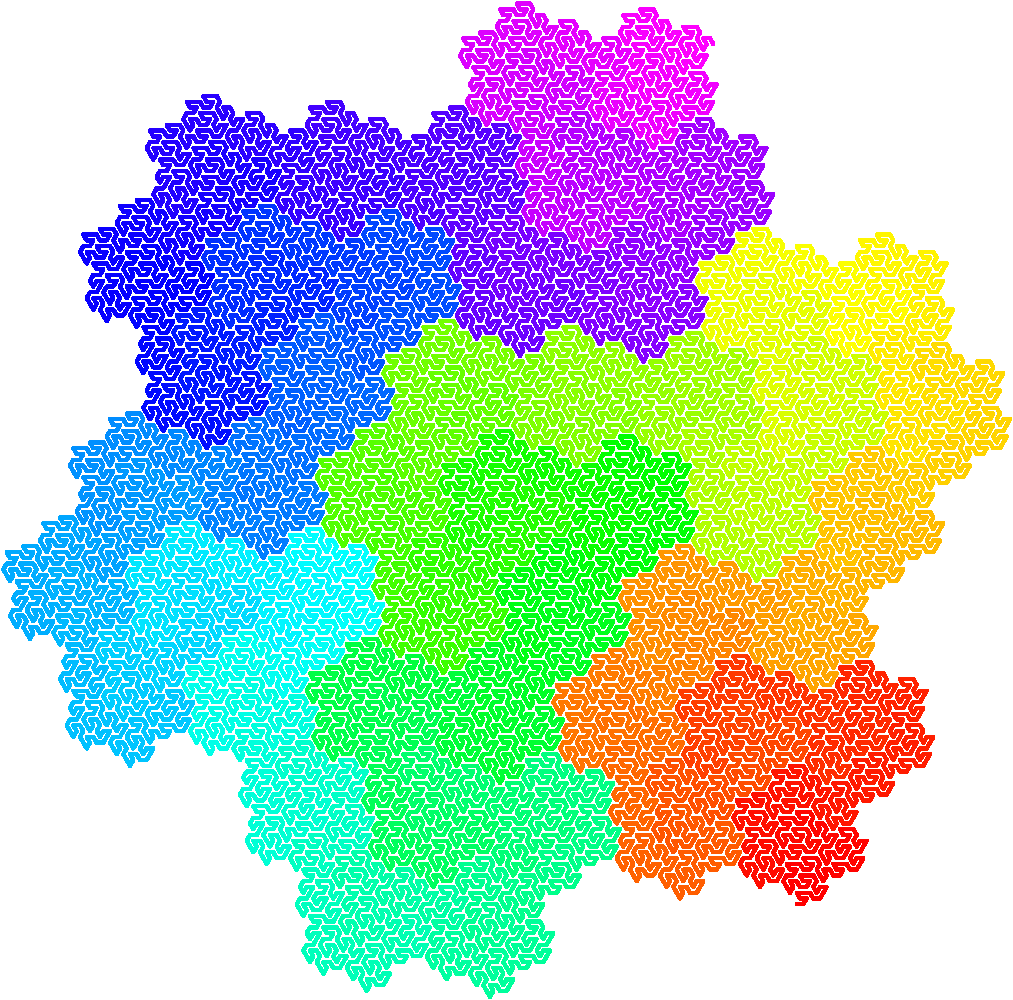
\includegraphics[width=	\linewidth]{HexaGosper}}
	\caption{Hexagonal Gosper curve}
\end{figure}

\newsavebox{\lstBoxGosper}
\begin{lrbox}{\lstBoxGosper}
\consolas
\footnotesize
\begin{lstlisting}
            ________          
            \       \         
  ________   \____   \        
  \       \      /   /        
   \____   \____/   /   ____  
       /            \   \   \ 
  ____/   ________   \   \   \
 /        \       \   \  /    
/   ____   \____   \   \/     
\   \   \      /   /          
 \   \   \____/   /   ____    
  \  /            \  /   /    
   \/   ________   \/   /     
        \       \      /      
         \____   \____/       
             /                
        ____/                 
\end{lstlisting}
\end{lrbox}

\begin{figure}[p]
	\subfloat{
		\minipage{0.47\linewidth}\noindent
			
\includegraphics[width=\linewidth]{HexaGosperFilled}
		\endminipage
	}
	\hfill
	\subfloat{
		\usebox{\lstBoxGosper}
	}
	\caption{Hexagonal Gosper curve as polygon (left) and as ASCII art (right)}
\end{figure}

\begin{figure}[p]
	\centering
	\subfloat{
\includegraphics[width=\linewidth]{IslandsAndLakes}}
	\caption{Islands and lakes}
\end{figure}

\begin{figure}[p]
	\subfloat{
\includegraphics[width=0.49\linewidth]{SierpinskiTriangle}}
	\hfill
	\subfloat{
\includegraphics[width=0.49\linewidth]{SierpinskiTriangleI}}
	\caption{Basic (left) and inverted (right) Sierpinski triangles}
\end{figure}

\begin{figure}[p]
	\centering
	\subfloat{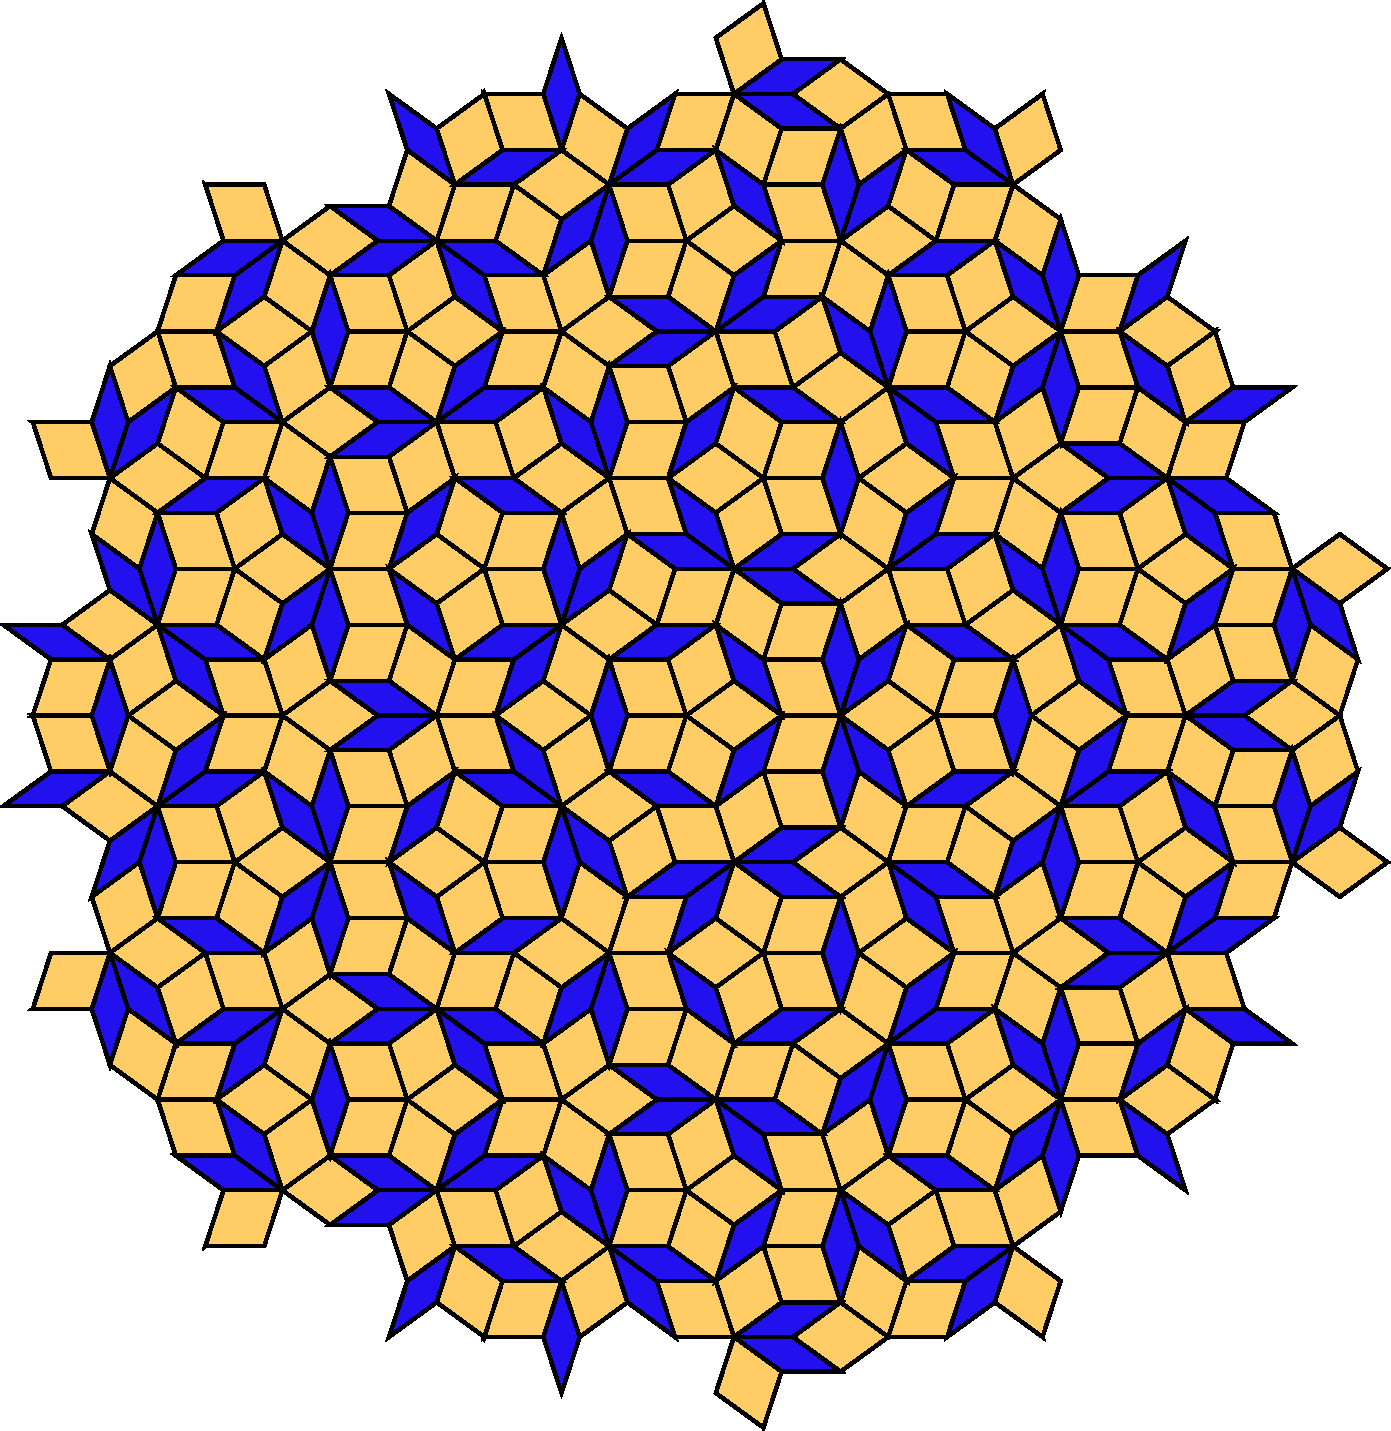
\includegraphics[width=\linewidth]{PenroseTiling}}
	\caption{Penrose tiling}
\end{figure}

\begin{figure}[p]
	\subfloat{
\includegraphics[width=0.40\linewidth]{Circles}}
	\hfill
	\subfloat{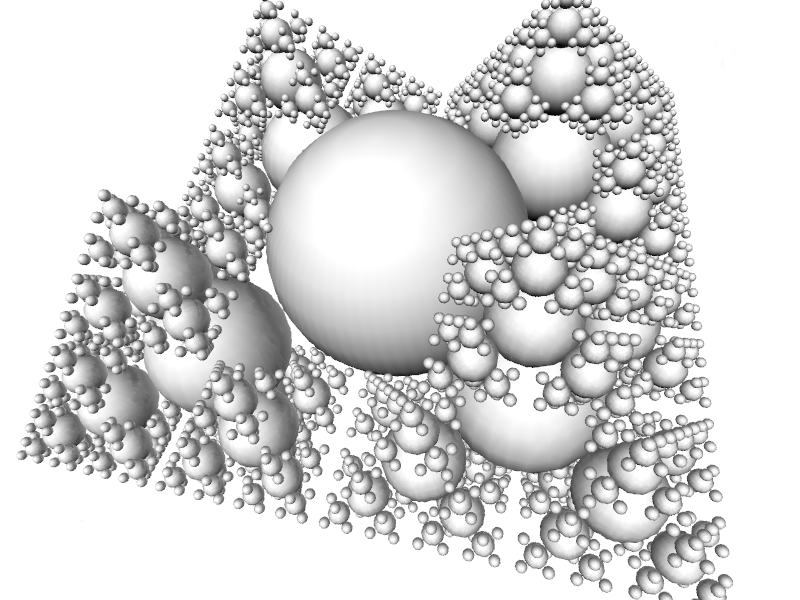
\includegraphics[width=0.58\linewidth]{Circles3D}}
	\caption{Circles (left) and its generalized version in 3D (right)}
\end{figure}

\begin{figure}[p]
	\centering
	\subfloat{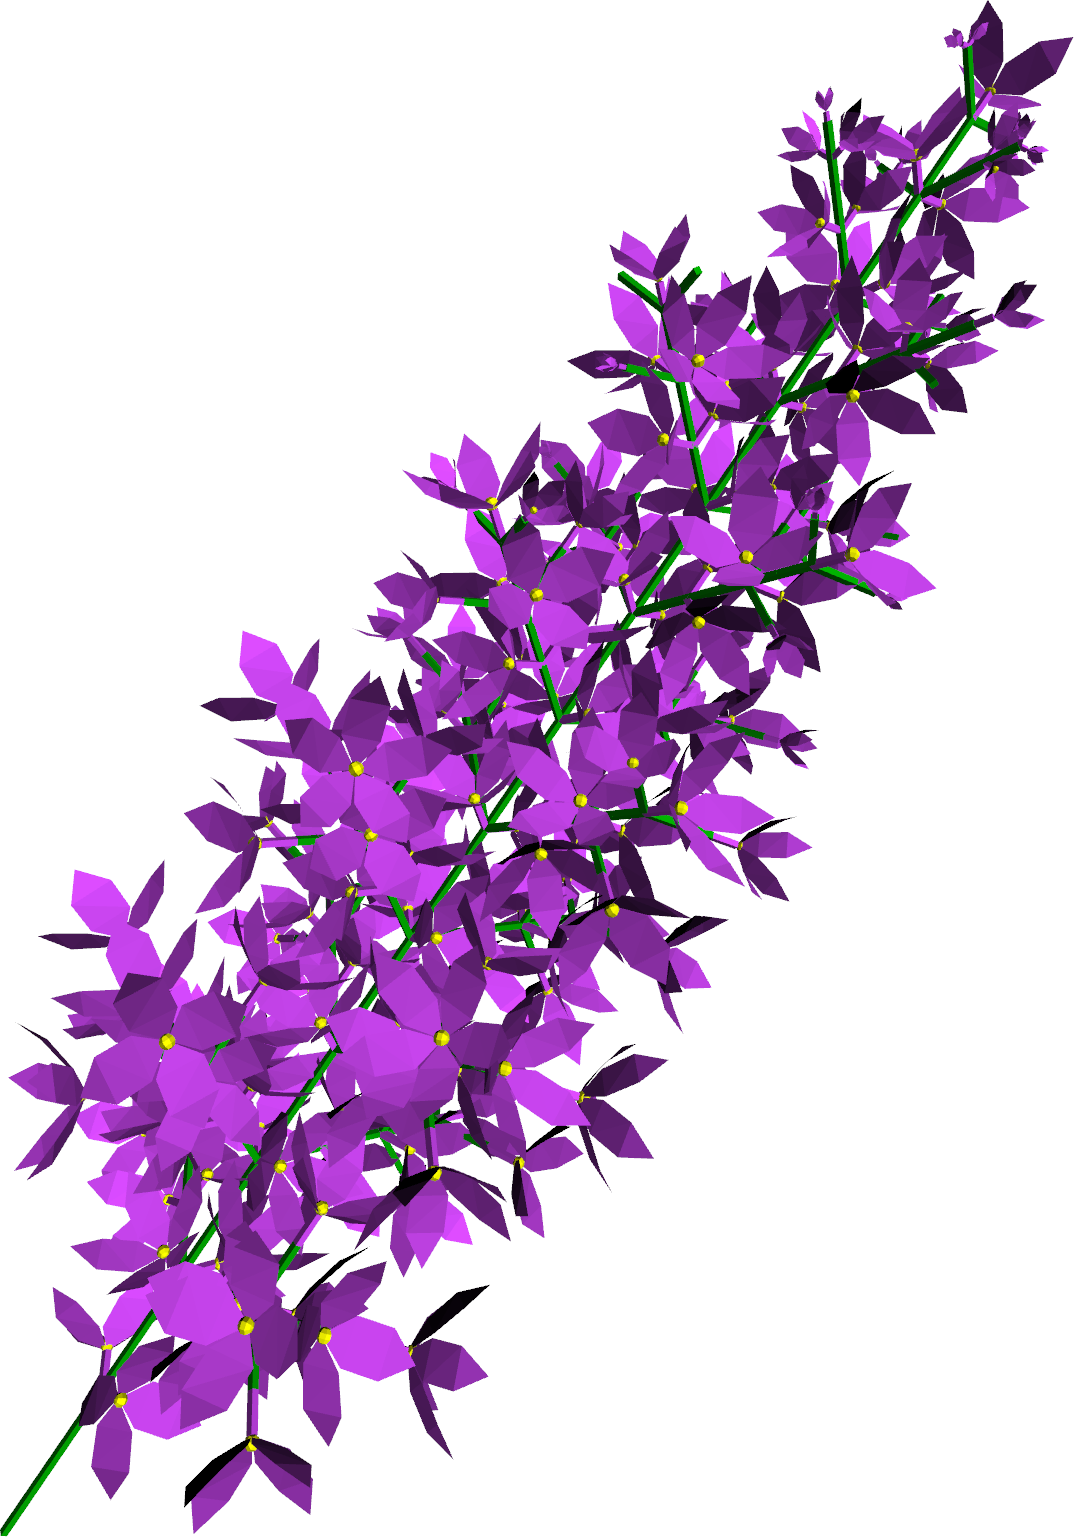
\includegraphics[width=\linewidth]{LilacHuge}}
	\caption{Lilac panicle}
\end{figure}

\begin{figure}[p]
	\centering
	\subfloat{
\includegraphics[width=\linewidth]{SunFlowerHuge}}
	\caption{Sunflower}
\end{figure}

\begin{figure}[p]
	\subfloat{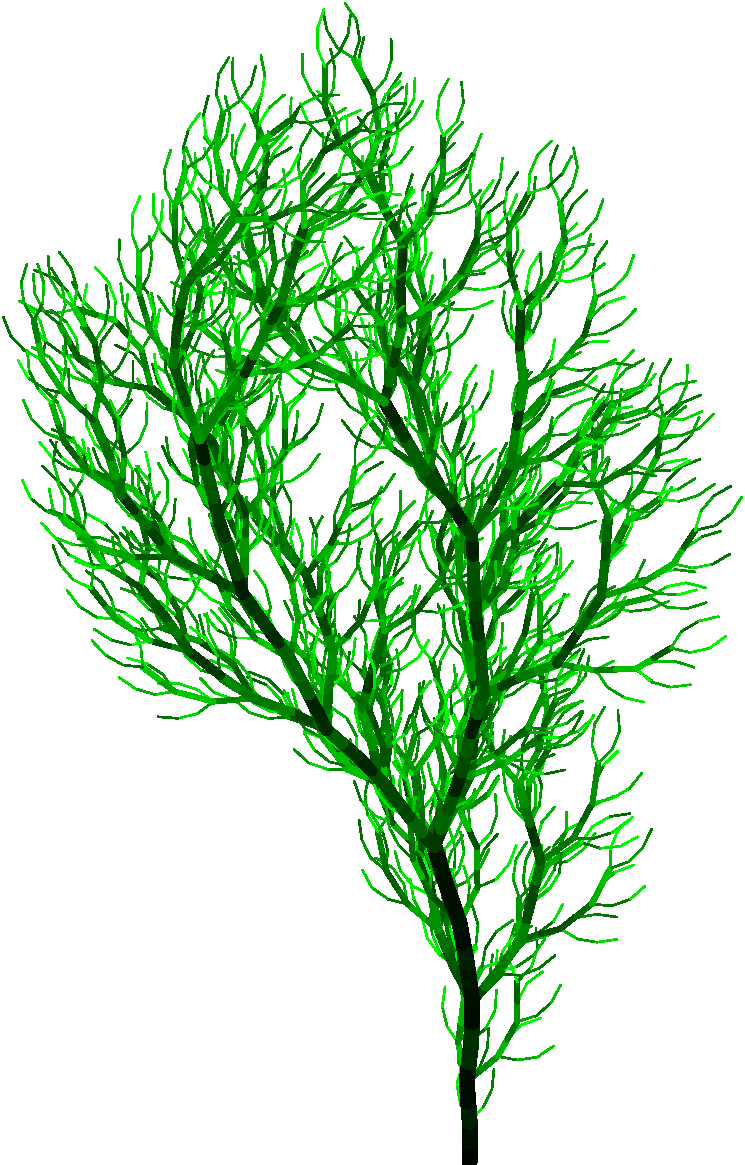
\includegraphics[width=0.28\linewidth]{Plant1}}
	\hfill
	\subfloat{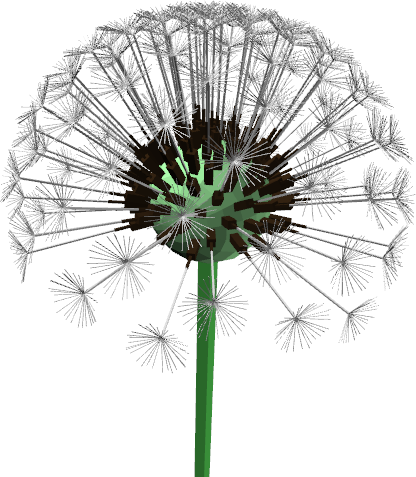
\includegraphics[width=0.36\linewidth]{Dandelion}}
	\hfill
	\subfloat{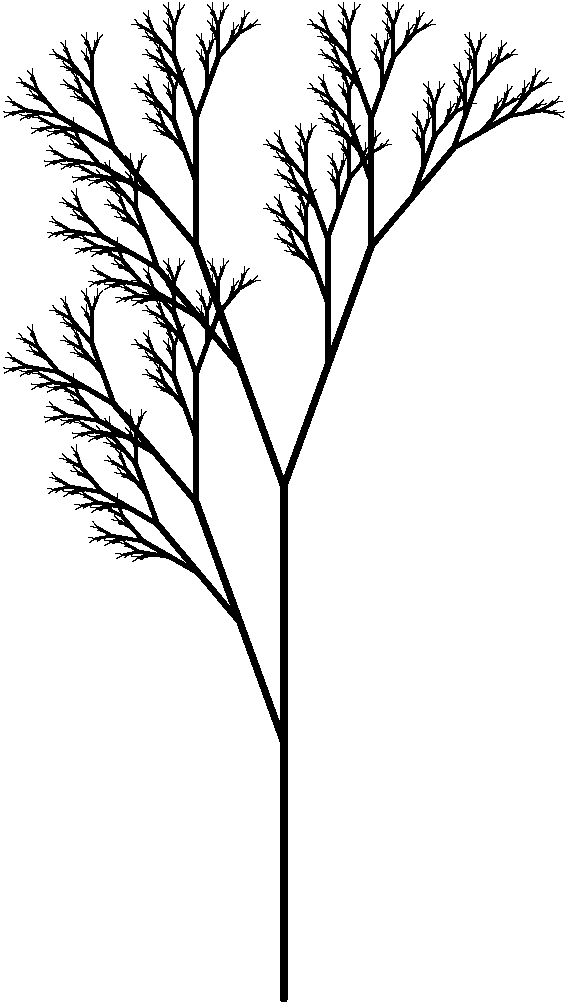
\includegraphics[width=0.25\linewidth]{Plant2}}
	\caption{Models of plant-like structures with withered dandelion in the middle}
\end{figure}



\section{Solution statistics}

\autoref{tbl:stats} shows number of lines of code written by hand based on file types.
Listed numbers do not include generated code (if not stated otherwise).
Also note that help pages with \emph{predefined stuff} in the web are generated dynamically thus their content is not included in statistics of total line count.


\begin{table}[h]
	\centering
	\begin{tabular}{p{65pt} c c p{200pt}}
   		\toprule
   		Extension & Type & Line count & Comment\\
   		\midrule
		.cs & C\# & > 30 000 &  \\ \hline
		.fs, .fsy, .fls & F\# & > 1 000 & F\# files together with lexer and parser definitions \\ \hline
		.cshtml & Razor & > 10 000 & views of the razor view engine\\ \hline
		.generated.cs, .designer.cs & C\# & > 5 000 & automatically generated files \\
		\bottomrule
	\end{tabular}
	\caption{Number of lines of code written by hand (if not stated otherwise) based on file types}
	\label{tbl:stats}
\end{table}























